\section{CW 复形的上同调}
\sourcepage{343}
现在可计算一些熟悉空间的上同调群，并找出代表其生成元的具体上闭链。基本工具如下。

\entry{定理}{5.8.1}若 $X$ 是 CW 复形，$\mathcal D(X)$ 是其胞腔链复形，则对任意 $p,G$，
\[
H^p(\mathcal D(X);G)\cong H^p(X;G).
\]
若 $X$ 可由复形 $K$ 三角剖分，则此同构由包含映射 $\mathcal D(X)\to\mathcal C(K)$ 诱导，方向与链映射相反。

\textbf{证明：}胞腔链复形与奇异链复形都自由，且同调同构，由推论 5.6.7，上同调也同构。可三角剖分时，定理 4.13.9 说明包含映射诱导同调同构，因此也诱导上同调同构。\hfill$\square$

\entry{推论}{5.8.2}设 $n>0$。有 $H^i(S^n;G)\cong G$（$i=0,n$），$H^i(B^n,S^{n-1};G)\cong G$（$i=n$），其余维数均为零。

\textbf{证明：}球面的胞腔链复形仅在零维及 $n$ 维为无限循环群，所有边缘为零，得到第一结论。再由球可缩及约化上同调长正合列，得到第二结论。\hfill$\square$

\sourcepage{344}
\entry{例}{5.8.3}环面 $T$ 与 Klein 瓶 $S$ 的胞腔链复形均具有形式
\[
0\to\Z\xrightarrow{\partial_2}\Z\oplus\Z\xrightarrow{\partial_1}\Z\to0.
\]
取二维生成元 $\gamma$，一维基 $w_1,z_1$。环面的所有边缘均为零，所以
\[
H^2(T;G)\cong G,\qquad H^1(T;G)\cong G\oplus G,\qquad H^0(T;G)\cong G.
\]
Klein 瓶满足 $\partial_1=0$、$\partial_2\gamma=2z_1$。在一维对偶群 $G\oplus G$ 中，第一项是只在 $w_1$ 上可能非零的同态，第二项是只在 $z_1$ 上可能非零的同态。上边缘在第一项上为零，在第二项上为乘以 $2$。因此
\[
H^2(S;G)\cong G/2G,\qquad H^1(S;G)\cong G\oplus\ker(G\xrightarrow{2}G),\qquad H^0(S;G)\cong G.
\]
特别地，整数系数时为 $H^2(S)\cong\Z/2$、$H^1(S)\cong\Z$、$H^0(S)\cong\Z$；模二系数时为 $H^2(S;\Z/2)\cong\Z/2$、$H^1(S;\Z/2)\cong(\Z/2)^2$、$H^0(S;\Z/2)\cong\Z/2$。\translatornote{原书模二公式的最后一项漏写了系数 $\Z/2$。}

一旦知道胞腔链复形，群的计算就不难。但要找出具体的\emph{单纯上闭链}代表生成元，则较困难；下一节计算杯积时将需要它们。

\sourcepage{345}
\begin{center}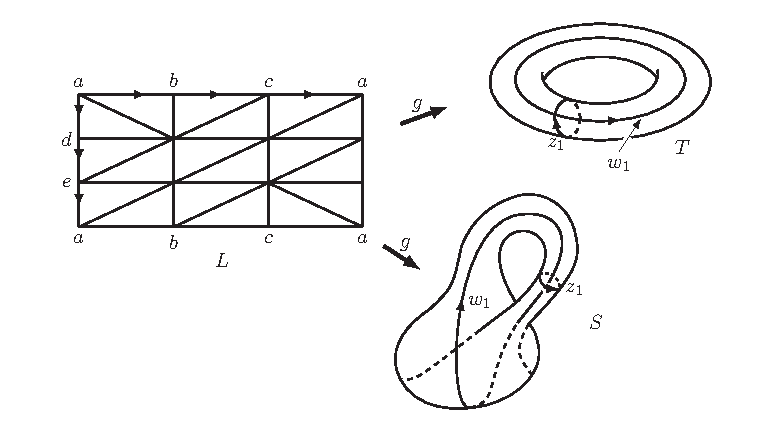
\includegraphics[width=.96\textwidth]{figures/5-8-1.pdf}\\图 5.8.1\end{center}
同调中，生成闭链容易找到：矩形中全部逆时针二维单形之和 $d$ 的像 $\gamma=g_\#d$ 生成 $D_2(X)$；链
\[
w_1=[a,b]+[b,c]+[c,a],\qquad z_1=[a,d]+[d,e]+[e,a]
\]
是 $D_1(X)$ 的基。胞腔同调同构由包含诱导，所以它们作为单纯链仍代表相应同调类。

上同调则不同。定义 $\lambda:D_2(X)\to\Z$ 使 $\lambda(\gamma)=1$；定义 $\varphi,\psi:D_1(X)\to\Z$，使
\[
\langle\varphi,w_1\rangle=1,\quad\langle\varphi,z_1\rangle=0,\qquad
\langle\psi,w_1\rangle=0,\quad\langle\psi,z_1\rangle=1.
\]
环面中，$\lambda$ 生成二维胞腔上同调，$\varphi,\psi$ 为一维基。Klein 瓶中，$\delta\varphi=0$、$\delta\psi=2\lambda$，故 $\lambda$ 代表二维非零类，$\varphi$ 代表一维生成元。

\sourcepage{346}
这些定义域只是胞腔链群，不能直接视为整个单纯复形上的上闭链，因为包含 $i:D_p(X)\to C_p(X)$ 的对偶是反向的限制映射。必须找到定义于所有单纯链上的上闭链，限制后等于 $\lambda,\varphi,\psi$，或代表它们的上同调类。一般没有现成的寻找程序；本例借助“栅栏”的直观可以找到。

\entry{例}{5.8.4（环面上同调的生成元）}图 5.8.2 中的上链 $w^1,z^1$ 直接计算可知上闭，且
\[
\langle w^1,w_1\rangle=1,\quad\langle w^1,z_1\rangle=0,\qquad
\langle z^1,w_1\rangle=0,\quad\langle z^1,z_1\rangle=1.
\]
所以它们限制后分别为 $\varphi,\psi$，代表 $H^1(T)$ 的一组基。任取逆时针定向二维单形 $\sigma$，则 $\sigma^*$ 上闭，且 $\langle\sigma^*,\gamma\rangle=1$，故限制为 $\lambda$，代表 $H^2(T)$ 的生成元。更一般地，$\sum n_i\sigma_i^*$ 的限制为 $\lambda$ 当且仅当 $\sum n_i=1$。

\sourcepage{347}
\begin{center}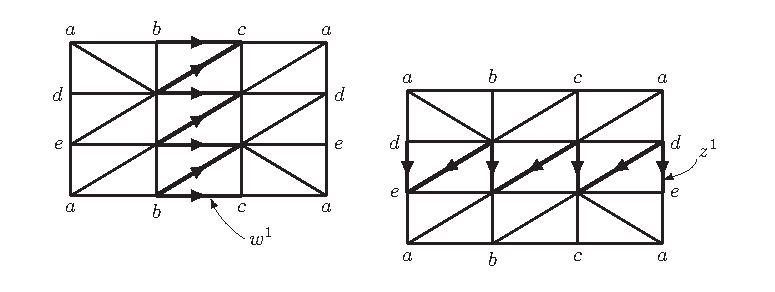
\includegraphics[width=.96\textwidth]{figures/5-8-2.pdf}\\图 5.8.2\end{center}
\entry{例}{5.8.5（Klein 瓶的整数上同调生成元）}交换图 5.8.2 中表示 $w^1$ 的矩形右侧标号 $d,e$，得到图 5.8.3。上链 $w^1$ 仍上闭，并生成 $H^1(S)$。任一二维初等上链 $\sigma^*$ 代表 $H^2(S)$ 的非零类。更一般地，若沿矩形全部二维单形取逆时针定向，则 $\sum n_i\sigma_i^*$ 代表非零类当且仅当系数和为奇数。
\begin{center}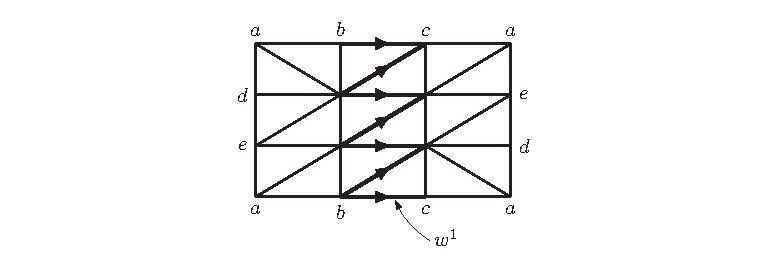
\includegraphics[width=.96\textwidth]{figures/5-8-3.pdf}\\图 5.8.3\end{center}

\entry{例}{5.8.6（Klein 瓶的模二上同调生成元）}按照同样论证，图 5.8.4 的 $w^1,z^1$ 生成二维向量空间 $H^1(S;\Z/2)$。图中不画箭头，因为模二时 $1=-1$。任一 $\sigma^*$，或奇数个不同初等二维上链之和，生成 $H^2(S;\Z/2)$。

\sourcepage{348}
\begin{center}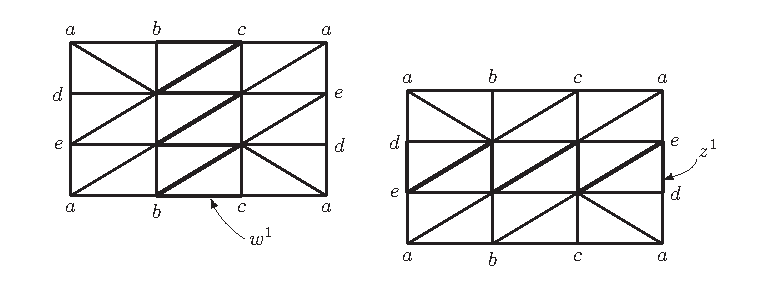
\includegraphics[width=.96\textwidth]{figures/5-8-4.pdf}\\图 5.8.4\end{center}
\entry{例}{5.8.7（实射影平面的模二上同调）}$H^i(P^2;\Z/2)\cong\Z/2$，$i=0,1,2$。二维初等上链代表二维生成元。图 5.8.5 的一维上闭链在胞腔生成闭链
\[
[a,b]+[b,c]+[c,d]+[d,e]+[e,f]+[f,a]
\]
上取值为 $1$，所以代表 $H^1(P^2;\Z/2)$ 的生成元。
\begin{center}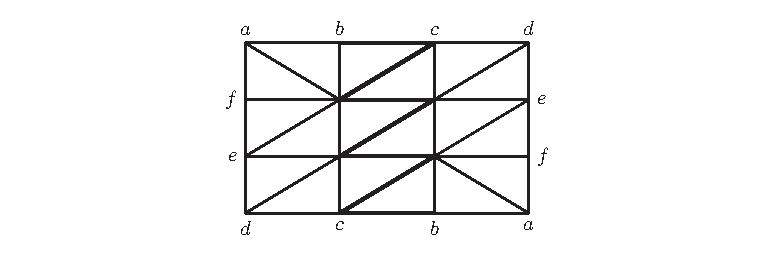
\includegraphics[width=.96\textwidth]{figures/5-8-5.pdf}\\图 5.8.5\end{center}

\sourcepage{349}
\subsection*{习题}
\begin{enumerate}
\item 分别用整数、模二、有理系数计算 $P^n,P^\infty$ 的上同调。
\item 计算 $\mathbb CP^n,\mathbb CP^\infty$ 的上同调。
\item 计算 $H^i(T\#T)$；采用第 1.7 节习题的三角剖分，找出生成上同调的单纯上闭链。
\item 计算四个实射影平面连通和的模二上同调，并找出生成上闭链。
\item 计算 Klein 瓶的 $\Z/6$ 系数上同调，仿照例 5.8.5、5.8.6 找代表上闭链。
\item 计算五重愚人帽的整数及 $\Z/5$ 系数上同调（第 1.7 节习题 6），三角剖分后找生成上闭链。
\item 计算 $L(n,k)$ 的整数及 $\Z/n$ 系数上同调。
\item 三角剖分 $S^2,T$，设 $f:T\to S^2$ 单纯。若 $f_*:H_2(T)\to H_2(S^2)$ 为乘以 $d$，通过比较生成元上取值，证明 $f^*:H^2(S^2)\to H^2(T)$ 也为乘以 $d$。与第 5.6 节习题 3 比较。
\item 计算环面的 $\Z/6$ 系数上同调。
\end{enumerate}
